\section{Methodology}\label{sec:method}
The elements of the Mandelbrot set are computed by the recursive function \code{iterate} that follows:

\begin{lstlisting}[language=C]
int iterate( float cx, float cy )
{
  float x = 0.0f, y = 0.0f, xnew, ynew;
  int it;
  for ( it = 0; (it < MAXIT) && (x*x + y*y <= 2.0*2.0); it++ ) {
    xnew = x*x - y*y + cx;
    ynew = 2.0*x*y + cy;
    x = xnew;
    y = ynew;
  }
  return it;
}
\end{lstlisting}

\noindent
Calling such function has a highly variable computational cost that depends on the number of loop iterations that, in turn, depends on the values of \code{cx} and \code{cy}, and on the maximum number of iterations allowed (\code{MAXIT}). In \code{omp-mandelbrot.c}, the \code{iterate} function is called within a two-level nested loop that computes the Mandelbrot set for a 2-D array having 768 rows (\code{y\_size}) and 1024 columns (\code{x\_size}), while the maximum number of iterations is set to 10000.

For the studies of this project, a new set of scripts\footnote{All scripts, data and images produced for this project are available at \href{https://github.com/mbarbetti/ppf-omp-project}{\code{mbarbetti/ppf-omp-project}}.} has been prepared, starting from a new source code, named \code{my-mandelbrot.c}. The main difference with respect to \code{omp-mandelbrot.c} is the memory allocation to store the elements of the Mandelbrot set, in order to export them for graphical visualization (see Figure \ref{fig:mandelbrot}). 

\begin{figure}[b!]
    \centering
    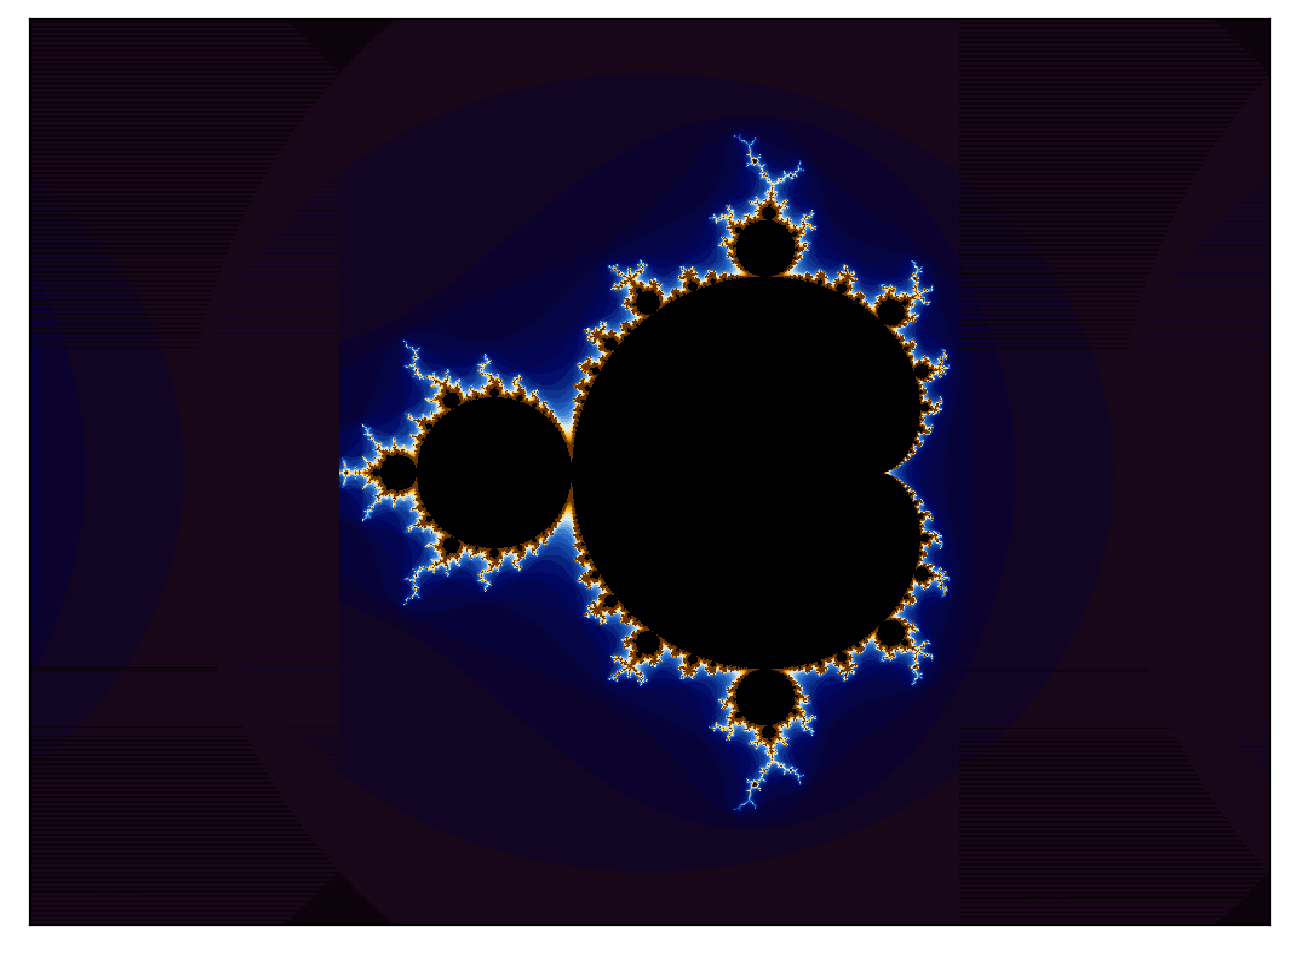
\includegraphics[width=0.99\textwidth]{mandelbrot.png}
    \caption{\label{fig:mandelbrot}}
\end{figure}

The program is parallelized using a set of OpenMP APIs that wraps the nested loop as shown in the following:

\newpage

\begin{lstlisting}[language=C]
  // [...]
#pragma omp parallel for private(x) schedule(runtime)
  for ( y = 0; y < y_size; y++ ) {
    for ( x = 0; x < x_size; x++ ) {
      const double re = x_min + (x_max - x_min) * (float)(x) / (x_size - 1);
      const double im = y_max - (y_max - y_min) * (float)(y) / (y_size - 1);
      const int it = iterate(re, im);   // highly variable work
#pragma omp critical
	  if ( it < MAXIT ) {
	    matrix[y*y_size + x] = it;   // saved for visualization
      }
    }
  }
  // [...]
\end{lstlisting}

\noindent
The use of the \codeblue{omp for} directive and of a private scope for the \code{x} variable means that only the inner loop is parallelized and its work distributed across the threads assigned the executing program by the \codeblue{omp parallel} directive. The time needed for completing the nested loop is measured (namely, the \emph{elapsed time}) and used performance studies.

In addition to the single-loop parallelization 



\begin{lstlisting}[language=C]
  // [...]
#pragma omp parallel for collapse(2) schedule(runtime)
  // [...]
\end{lstlisting}

\subsection{Scheduling study}\label{sec:method-sched}

\subsection{Scaling study}\label{sec:method-scale}